\documentclass[11pt, A4paper]{article}
\usepackage[utf8]{inputenc}
\usepackage[left=3.15cm, right=3.15cm, top=3.15cm, bottom=3.15cm]{geometry}
\usepackage{multicol}
\usepackage[none]{hyphenat}
\usepackage{titlesec}
\usepackage{times}
\usepackage{indentfirst}
\usepackage{capt-of}%%To get the caption
\usepackage{gensymb}
\usepackage{graphicx} %package to manage images
\graphicspath{ {./images/} }
\usepackage{wrapfig}
\usepackage{lipsum} 

\usepackage{listings}
\lstset{
    %language=Python,
    basicstyle=\ttfamily\small,
    aboveskip={1.0\baselineskip},
    belowskip={1.0\baselineskip},
    columns=fixed,
    extendedchars=true,
    breaklines=true,
    tabsize=4,
    prebreak=\raisebox{0ex}[0ex][0ex]{\ensuremath{\hookleftarrow}},
    frame=lines,
    showtabs=false,
    showspaces=false,
    showstringspaces=false,
    keywordstyle=\color[rgb]{0.627,0.126,0.941},
    commentstyle=\color[rgb]{0.133,0.545,0.133},
    stringstyle=\color[rgb]{01,0,0},
    numbers=left,
    basicstyle = tiny
    numberstyle=\small,
    stepnumber=1,
    numbersep=10pt,
    captionpos=t,
    escapeinside={(*}{*)},
}

\usepackage{scalerel}

\usepackage{fancyhdr}
\pagestyle{fancy}
\fancyhf{}
\renewcommand{\headrulewidth}{0pt}
\fancyhead[R]{\textit{\large{\thepage}}}
\lhead{\normal{\textit{Qualification Round Reverse Engineering Challenge for HACK3D 2018}}}




\usepackage[backend=biber,style=apa,autocite=inline]{biblatex}
\DeclareLanguageMapping{english}{english-apa}

\addbibresource{references.bib}

\begin{document}

\titleformat*{\section}{\normal\bfseries}
\titlelabel{\thetitle.\quad}

\begingroup
\setlength{\parindent}{0pt}% Remove paragraph indent

\LARGE 
\bfseries 
\linespread{1} 
A New Method for Reverse Engineering XYZ coordinates into   Computer-Aided Design (CAD) and Stereolithography (STL) File Formats

\bigskip
\endgroup

{
\setlength{\parindent}{0pt}% Remove paragraph indent
\large
\bfseries Nishant Aswani, Barkin Simsek
\bigskip
}

{
\setlength{\parindent}{0pt}% Remove paragraph indent
\textit{16 October 2018}
}


\setlength\columnsep{15pt}
\begin{multicols}{2}


\section{Problem Identification and Statement}

The proposed challenge involved the reconstruction of a solid 3D model based on a given set of XYZ coordinates. The XYZ coordinates provided represented the nozzle movements of a 3D printer that printed at a layer thickness of 0.2 mm. The reconstruction was required to result in a stereolitography (.STL) file.



\section{Gathering Information and Object Visualization}

\begingroup
    \bigskip
    \centering
    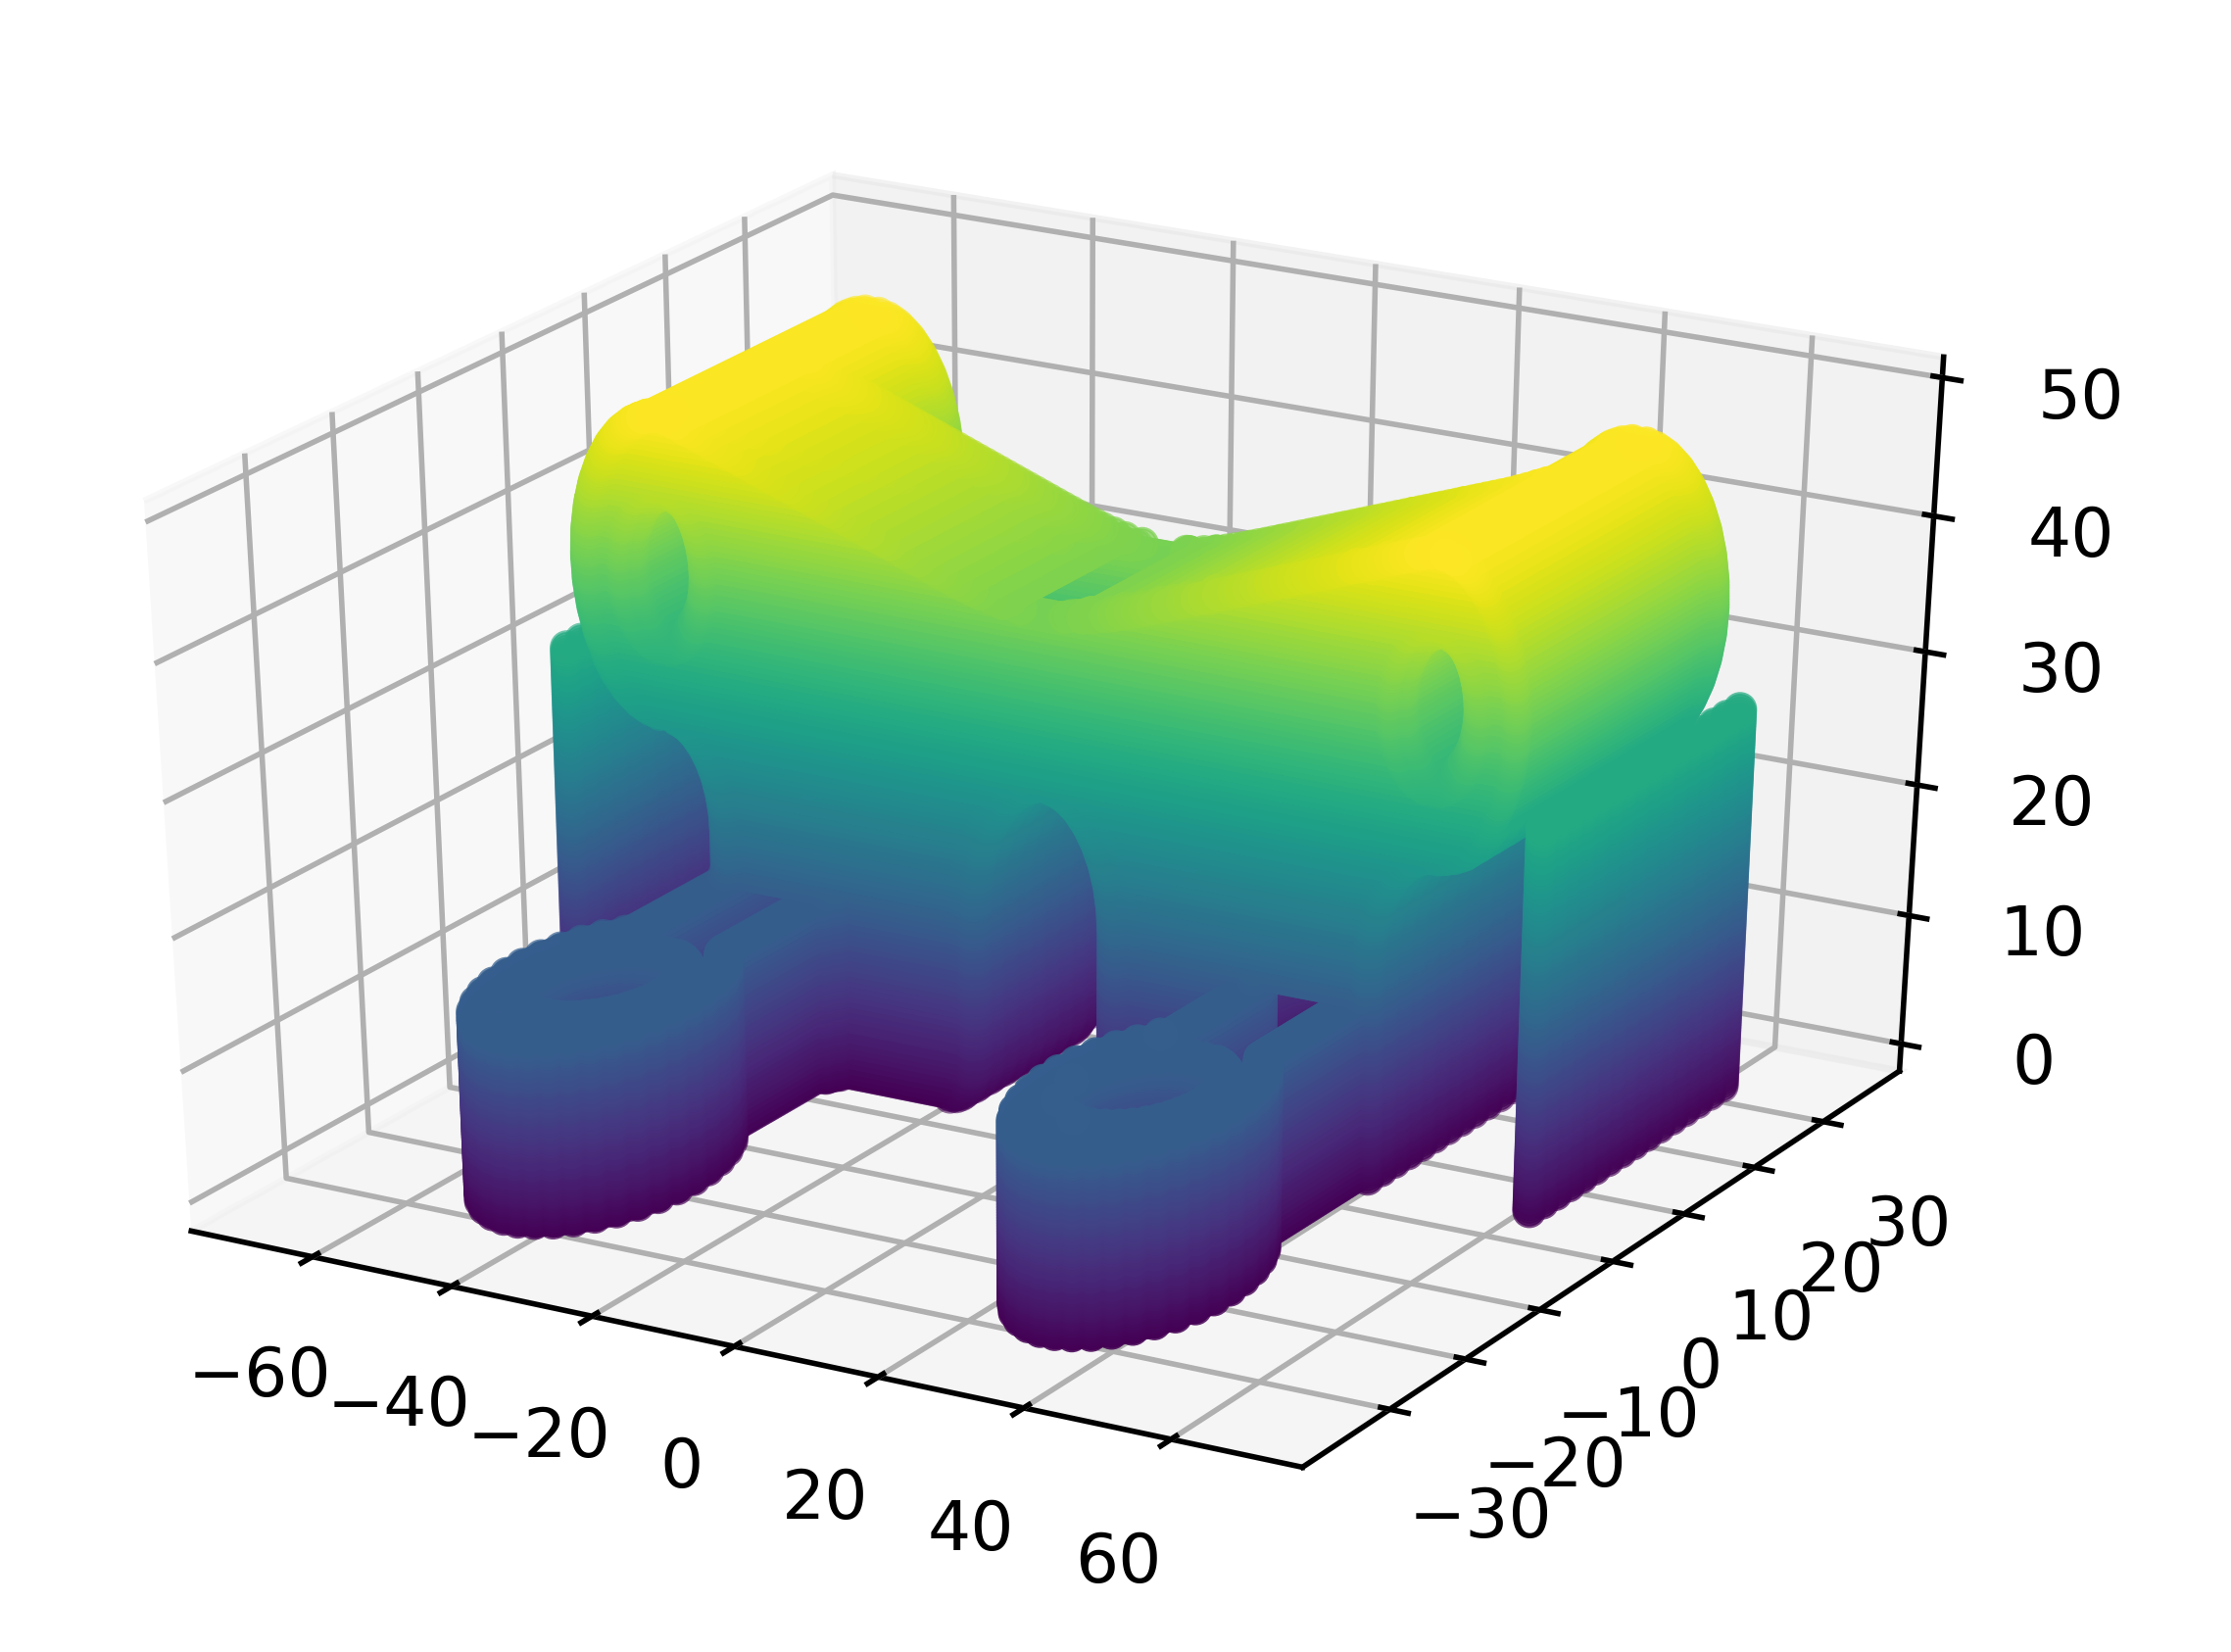
\includegraphics[width=\columnwidth]{scatter}
    \small{\captionof{figure}{A scatter plot visualization of the XYZ coordinates}}
    \label{fig:python_vis}
        \bigskip
\endgroup

In order to visualize and comprehend the final structure, the numpy library and scatter plot function in Python were implemented to produce a 3D graph. The individual plotting of points provided a structure dense enough to produce the structure depicted in Figure 1.

Processing the original .txt file made it easier to work with in Python. A header row was added to the .txt file denoting each column with it's respective descriptor (i.e. "x  coor" for x coordinates). The .txt file was then saved as a .csv file for use with the pandas library. The code used for the preliminary Python implementation can be founder under listing 1 in the Appendix.

\begingroup
    \bigskip
    \centering
    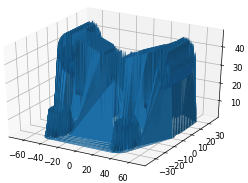
\includegraphics[width=\columnwidth]{trisurface}
    \small{\captionof{figure}{An attempted trisurface plot visualization of the XYZ coordinates}}
    \label{fig:trisurf_vis}
        \bigskip
\endgroup

Having visualized the data, it was hypothesized that there was some Python library,which would transform a set of XYZ coordinates into a 3D mesh, allowing one to export the mesh as an STL file. A tutorial blog post(\cite[]{stlblog}) described a Python library called "numpy-stl," capable of working with STL meshes. Looking at the documentation of numpy-stl (\cite[]{numpy-stl}), it was discovered that STL generation, at least for the library in question, would require vertices and faces. 

A numpy-stl issue ticket, found on the library's git page (\cite[]{stl-ticket}), inspired a new approach involving the use of triangulation to generate the 3D plot. This resulted in the trisurface plot depicted in Figure 2. However, due to the numerous unclean lines that were deforming the object, this approach was discarded. 

Other attempts at using libraries to directly generate an STL mesh from point coordinates involved separately employing the surf2stl library in Mathematica and pygmsh library in Python; however, these approaches too were to no avail.

Further research, and a new drive to understand the process, elucidated what occurs when a STL file is generated. Figure 3 explained the notion that an STL file is essentially a high-resolution polygon mesh of the CAD model. Moreover, a Stack Overflow answer outlined how one would go about constructing triangles from a set of given coordinates. Essentially, given a coordinate \ensuremath{P(i,j)}, one could connect it to another coordinate \ensuremath{P(i+x,j)}, then connect that to \ensuremath{P(i+x, j+x)} to form a clockwise triangle of three vectors. The next triangle, restricted to the clockwise orientation, could be formed by connecting the three points, \ensuremath{P(i,j)}, \ensuremath{P(i+x, j+x)}, and \ensuremath{P(i, j+x)} with vector lines. Finally, the normal could be generated by using the cross product from two vectors that were part of a triangle.

\section{Attempt at Using Meshlab}

Meshlab's features provided a potential work-around to the issue of creating triangles from XYZ coordinates. The program was capable of computing normals for point sets, as well as supporting Poisson surface reconstruction to create an mesh file (\cite[]{poisson}), which could eventually be saved as an STL file.

\begingroup
    \bigskip
    \centering
    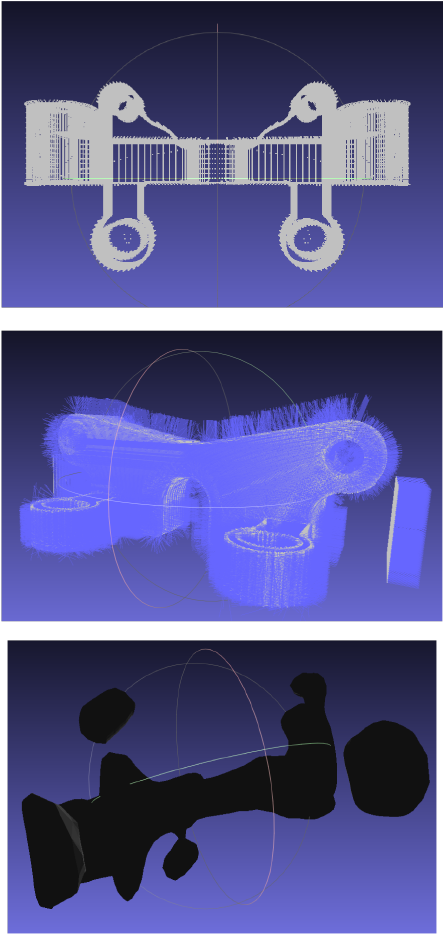
\includegraphics[width=\columnwidth]{meshlab}
    \small{\captionof{figure}{The top figure shows the imported point cloud. The middle figure displays the rendered normals. The final figure shows a variation of a a Poisson surface reconstruction.}}
    \label{fig:meshlab}
        \bigskip
\endgroup

Figure 4c shows one of the various attempts at the Poisson surface reconstruction, highlighting the abstract nature of and the difficulty that occurred in recreating the 3D structure in Meshlab. This process was concluded to be imprecise and not rigorous enough to generate a feasible STL file.

\begingroup
    \centering
    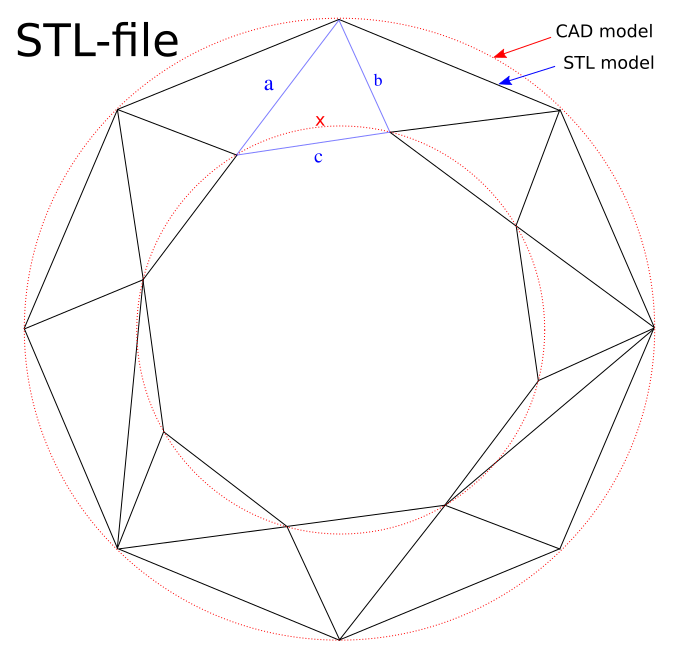
\includegraphics[width=\columnwidth]{cad-vs-stl}
    \small{\captionof{figure}{Two concentric circles, representing a CAD model of a doughnut shape, and a series of triangles approximating the doughnut, representing how STL modeling works.}}
    \label{fig:explainSTL}
\endgroup

\section{Onshape}

A final and successful attempt at recreating the 3D structure came about as a result of thinking through the lens of a slicer. Initially, openSCAD was used to draw polygons for each layer, extrude each layer, and shift the layers to their respective heights. Having automated this process in a few simple lines of code, it seemed the most efficient way of recreating the object. However, openSCAD does not allow for files to be imported; therefore, the coordinates had to be copied into the code, leading to a file that could not be reasonably executed. 

Certain that a CAD software would work, the FeatureScript component offered by Onshape was discovered. The FeatureScript tool, which allows one to design CAD models through JavaScript and C syntax, was used to automate the process of STL generation. The actions of creating a sketch, drawing a poly-line through all of the points on a given layer, deleting unnecessary faces, and then extruding the sketch by 2 millimeters were all automated for the 234 layers. 

The first attempt at using FeatureScript did not involve a mechanism to clean the unnecessary faces generated from the polyline drawing, thus a manual cleaning of the first layer was carried out.

\begingroup
    \bigskip
    \centering
    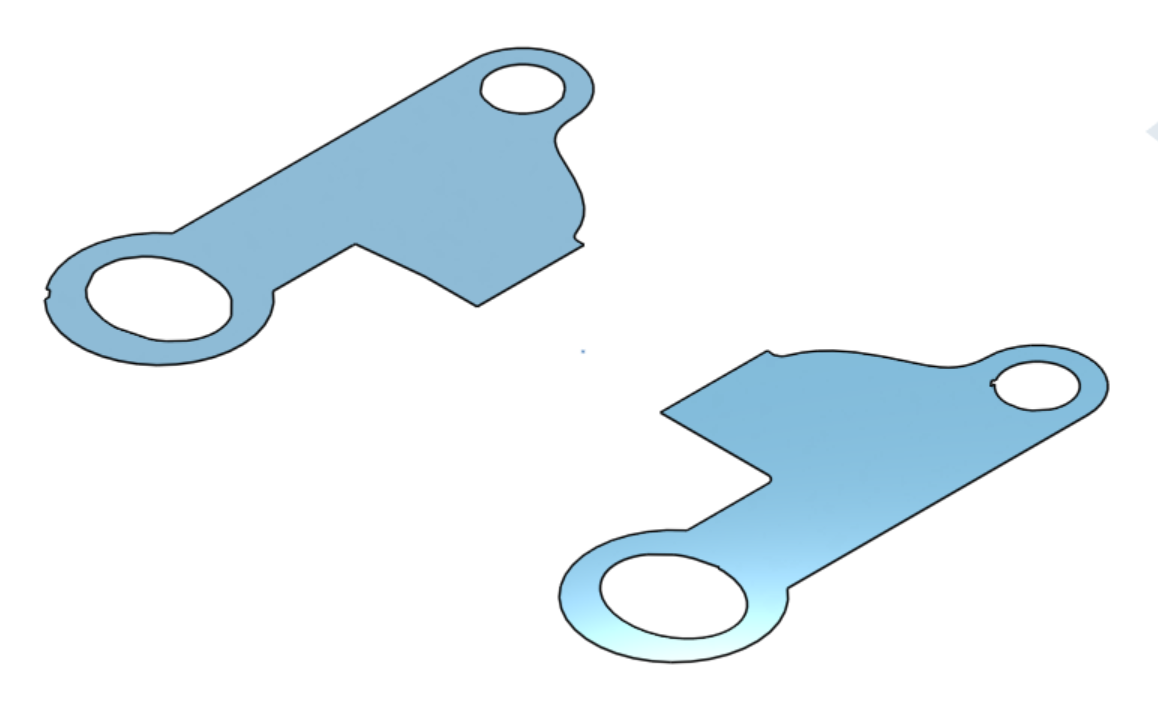
\includegraphics[width=\columnwidth]{onshape_one}
    \small{\captionof{figure}{The first layer regenerated in Onshape and manually cleaned.}}
    \label{fig:onshape_one}
        \bigskip
\endgroup

However, it was soon clear that manual cleaning and extrusion would not be feasible for a total of 234 layers. 

Thus, future versions of the FeatureScript code were developed to querying all the faces in a layer, querying the largest of them in a for loop, and deleting them before carrying out extrusion. While this did not result in sketches as well cleaned as in Figure 5, it allowed for a basic, automated cleaning for 234 layers. 

Onshape was unable to render and assemble all of the layers in one document for final touches and STL export. Thus, several layers were packaged and generated separately in Onshape (see Figure 6), all of which were exported and assembled in Autodesk Fusion 360. Figure 7 represents the final product. 

The Onshape script can be found within the compressed folder and is not listed in the appendix. 

\begingroup
    \bigskip
    \centering
    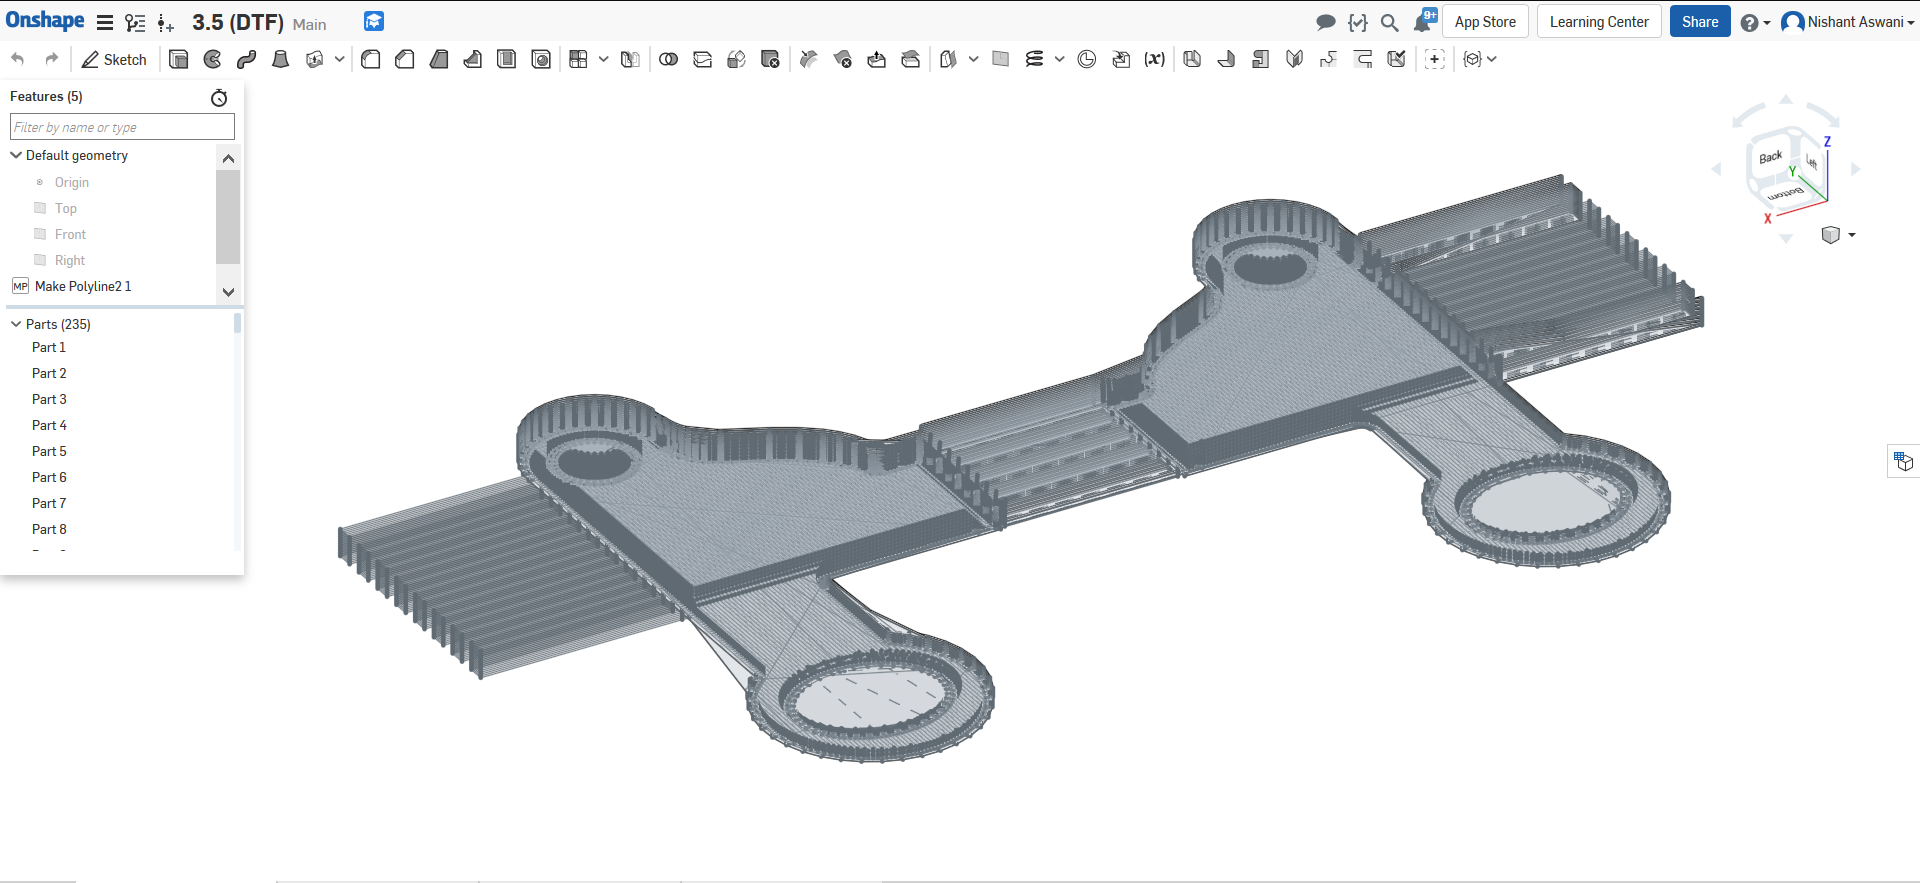
\includegraphics[width=\columnwidth]{onshape_two}
    \small{\captionof{figure}{Package 5, depicting a selection of layers found in the first third of the structure}}
    \label{fig:onshape_one}
        \bigskip
\endgroup

\section{Acknowledgements}
The Engineering Design Studio (EDS) for being our home, allowing us access to powerful resources, and providing a welcoming atmosphere.



Matthew Karau for his vision for engineering students and the EDS. 

Daniel Chirita and H. Utku Unlu for checking the logic of our code and acting as motivators and guides.

\printbibliography

\end{multicols}

\begingroup
    \bigskip
    \centering
    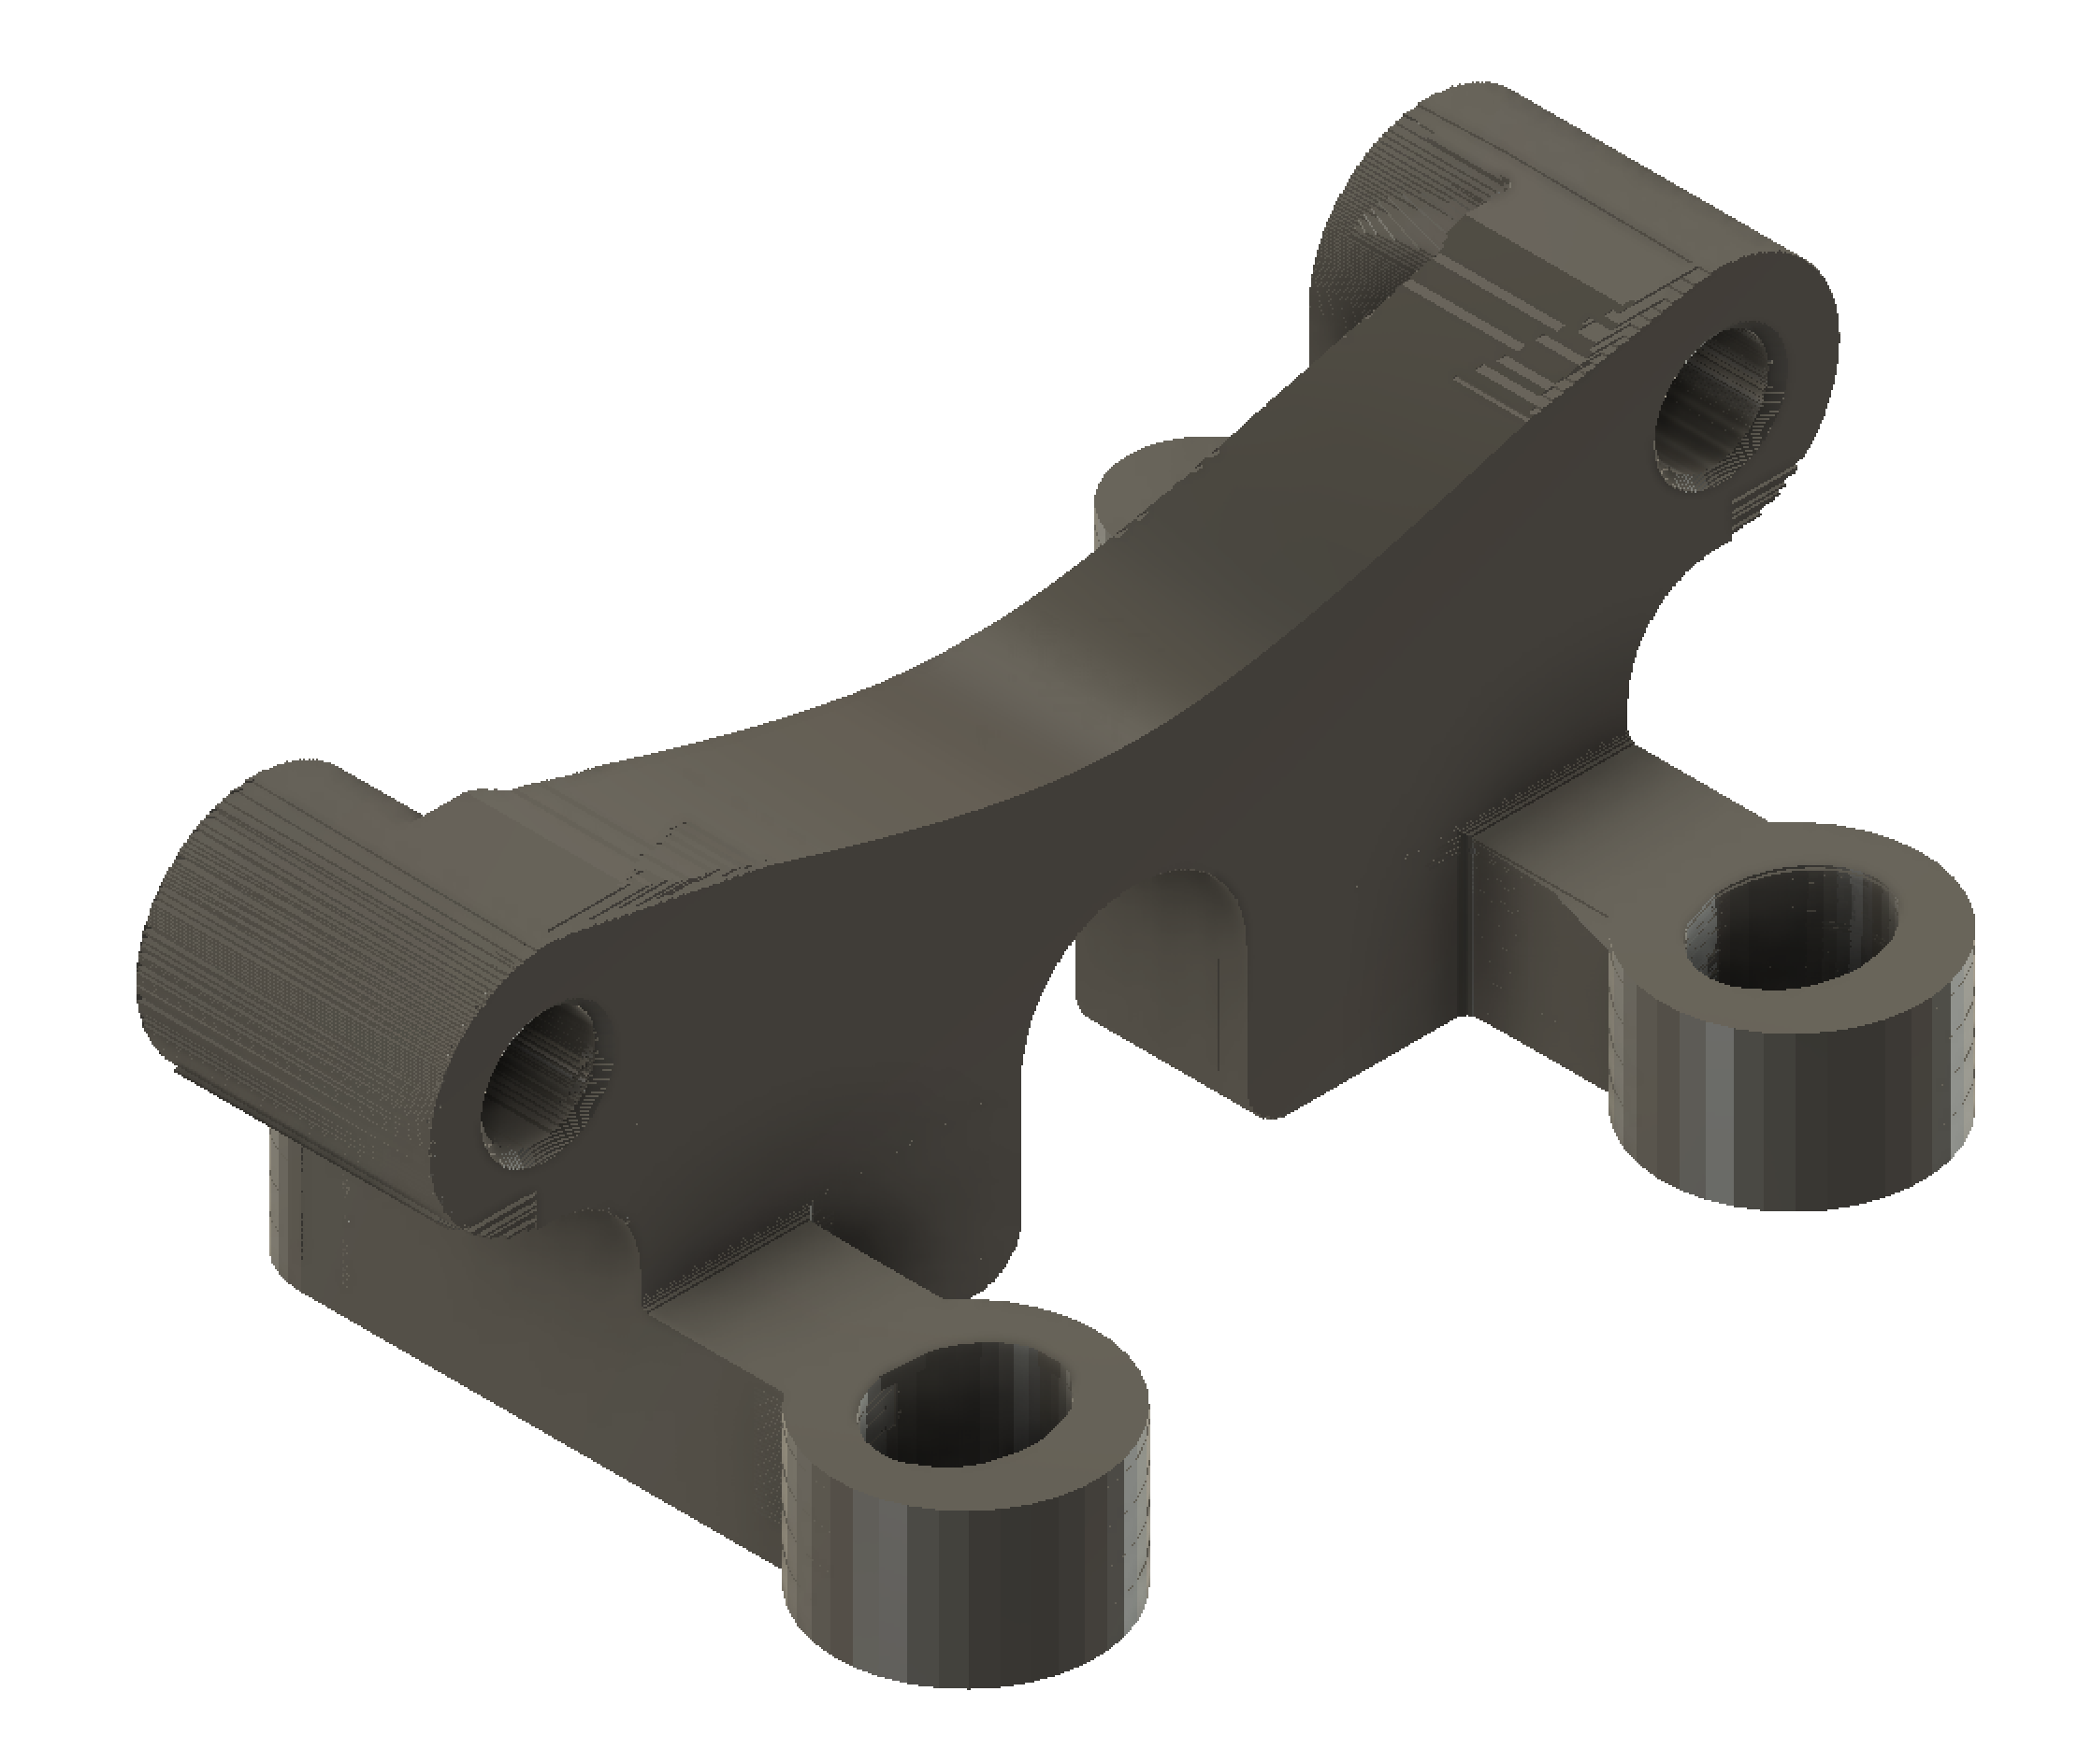
\includegraphics[scale = 0.3]{final}
    \small{\captionof{figure}{The final STL file}}
    \label{fig:final}
        \bigskip
\endgroup


\newpage
\section{Appendix}

\begin{lstlisting}[label={list:first},caption=Python Code for Visualization.]
from mpl_toolkits import mplot3d
import pandas as pd
import csv
import numpy as np
import matplotlib.pyplot as plt
%matplotlib inline

df = pd.read_csv('C:\\Users\\username\\Downloads\\xyz.txt',delimiter=\t)

a =df['x_coor'].values
x = a.tolist()

b =df['y_coor'].values
y = b.tolist()

c =df['z_coor'].values
z = c.tolist()

ax= plt.axes(projection='3d')
ax.scatter(x,y,z, c=z, cmap='virids', linewidth=0.5)

\end{lstlisting}














\end{document}